%!TEX TS-program = xelatex 
\documentclass[12pt, a4paper]{article} 

\usepackage{etex} % расширение классического tex в частности позволяет подгружать гораздо больше пакетов, чем мы и займёмся далее 

%%%%%%%%%% Математика %%%%%%%%%% 
\usepackage{amsmath,amsfonts,amssymb,amsthm,mathtools} 
%\mathtoolsset{showonlyrefs=true} % Показывать номера только у тех формул, на которые есть \eqref{} в тексте. 
%\usepackage{leqno} % Нумерация формул слева 


%%%%%%%%%%%%%%%%%%%%%%%% Шрифты %%%%%%%%%%%%%%%%%%%%%%%%%%%%%%%%% 
\usepackage{fontspec} % пакет для подгрузки шрифтов 
\setmainfont{Arial} % задаёт основной шрифт документа 

\defaultfontfeatures{Mapping=tex-text} 

% why do we need \newfontfamily: 
% http://tex.stackexchange.com/questions/91507/ 
\newfontfamily{\cyrillicfonttt}{Arial} 
\newfontfamily{\cyrillicfont}{Arial} 
\newfontfamily{\cyrillicfontsf}{Arial} 

\usepackage{unicode-math} % пакет для установки математического шрифта 
\setmathfont{Asana Math} % шрифт для математики 

\usepackage{polyglossia} % Пакет, который позволяет подгружать русские буквы 
\setdefaultlanguage{russian} % Основной язык документа 
\setotherlanguage{english} % Второстепенный язык документа 


%%%%%%%%%% Работа с картинками %%%%%%%%% 
\usepackage{graphicx} % Для вставки рисунков 
\usepackage{graphics} 
\usepackage{float} 
\graphicspath{{images/}{pictures/}} % можно указать папки с картинками 
\usepackage{wrapfig} % Обтекание рисунков и таблиц текстом 
\usepackage{subfigure} % для создания нескольких рисунков внутри одного 
\title{Задание 2.1}
\date{}
\begin{document} 
\maketitle
\begin{figure}[h!]
\begin{minipage}[h!]{0.28\linewidth} 
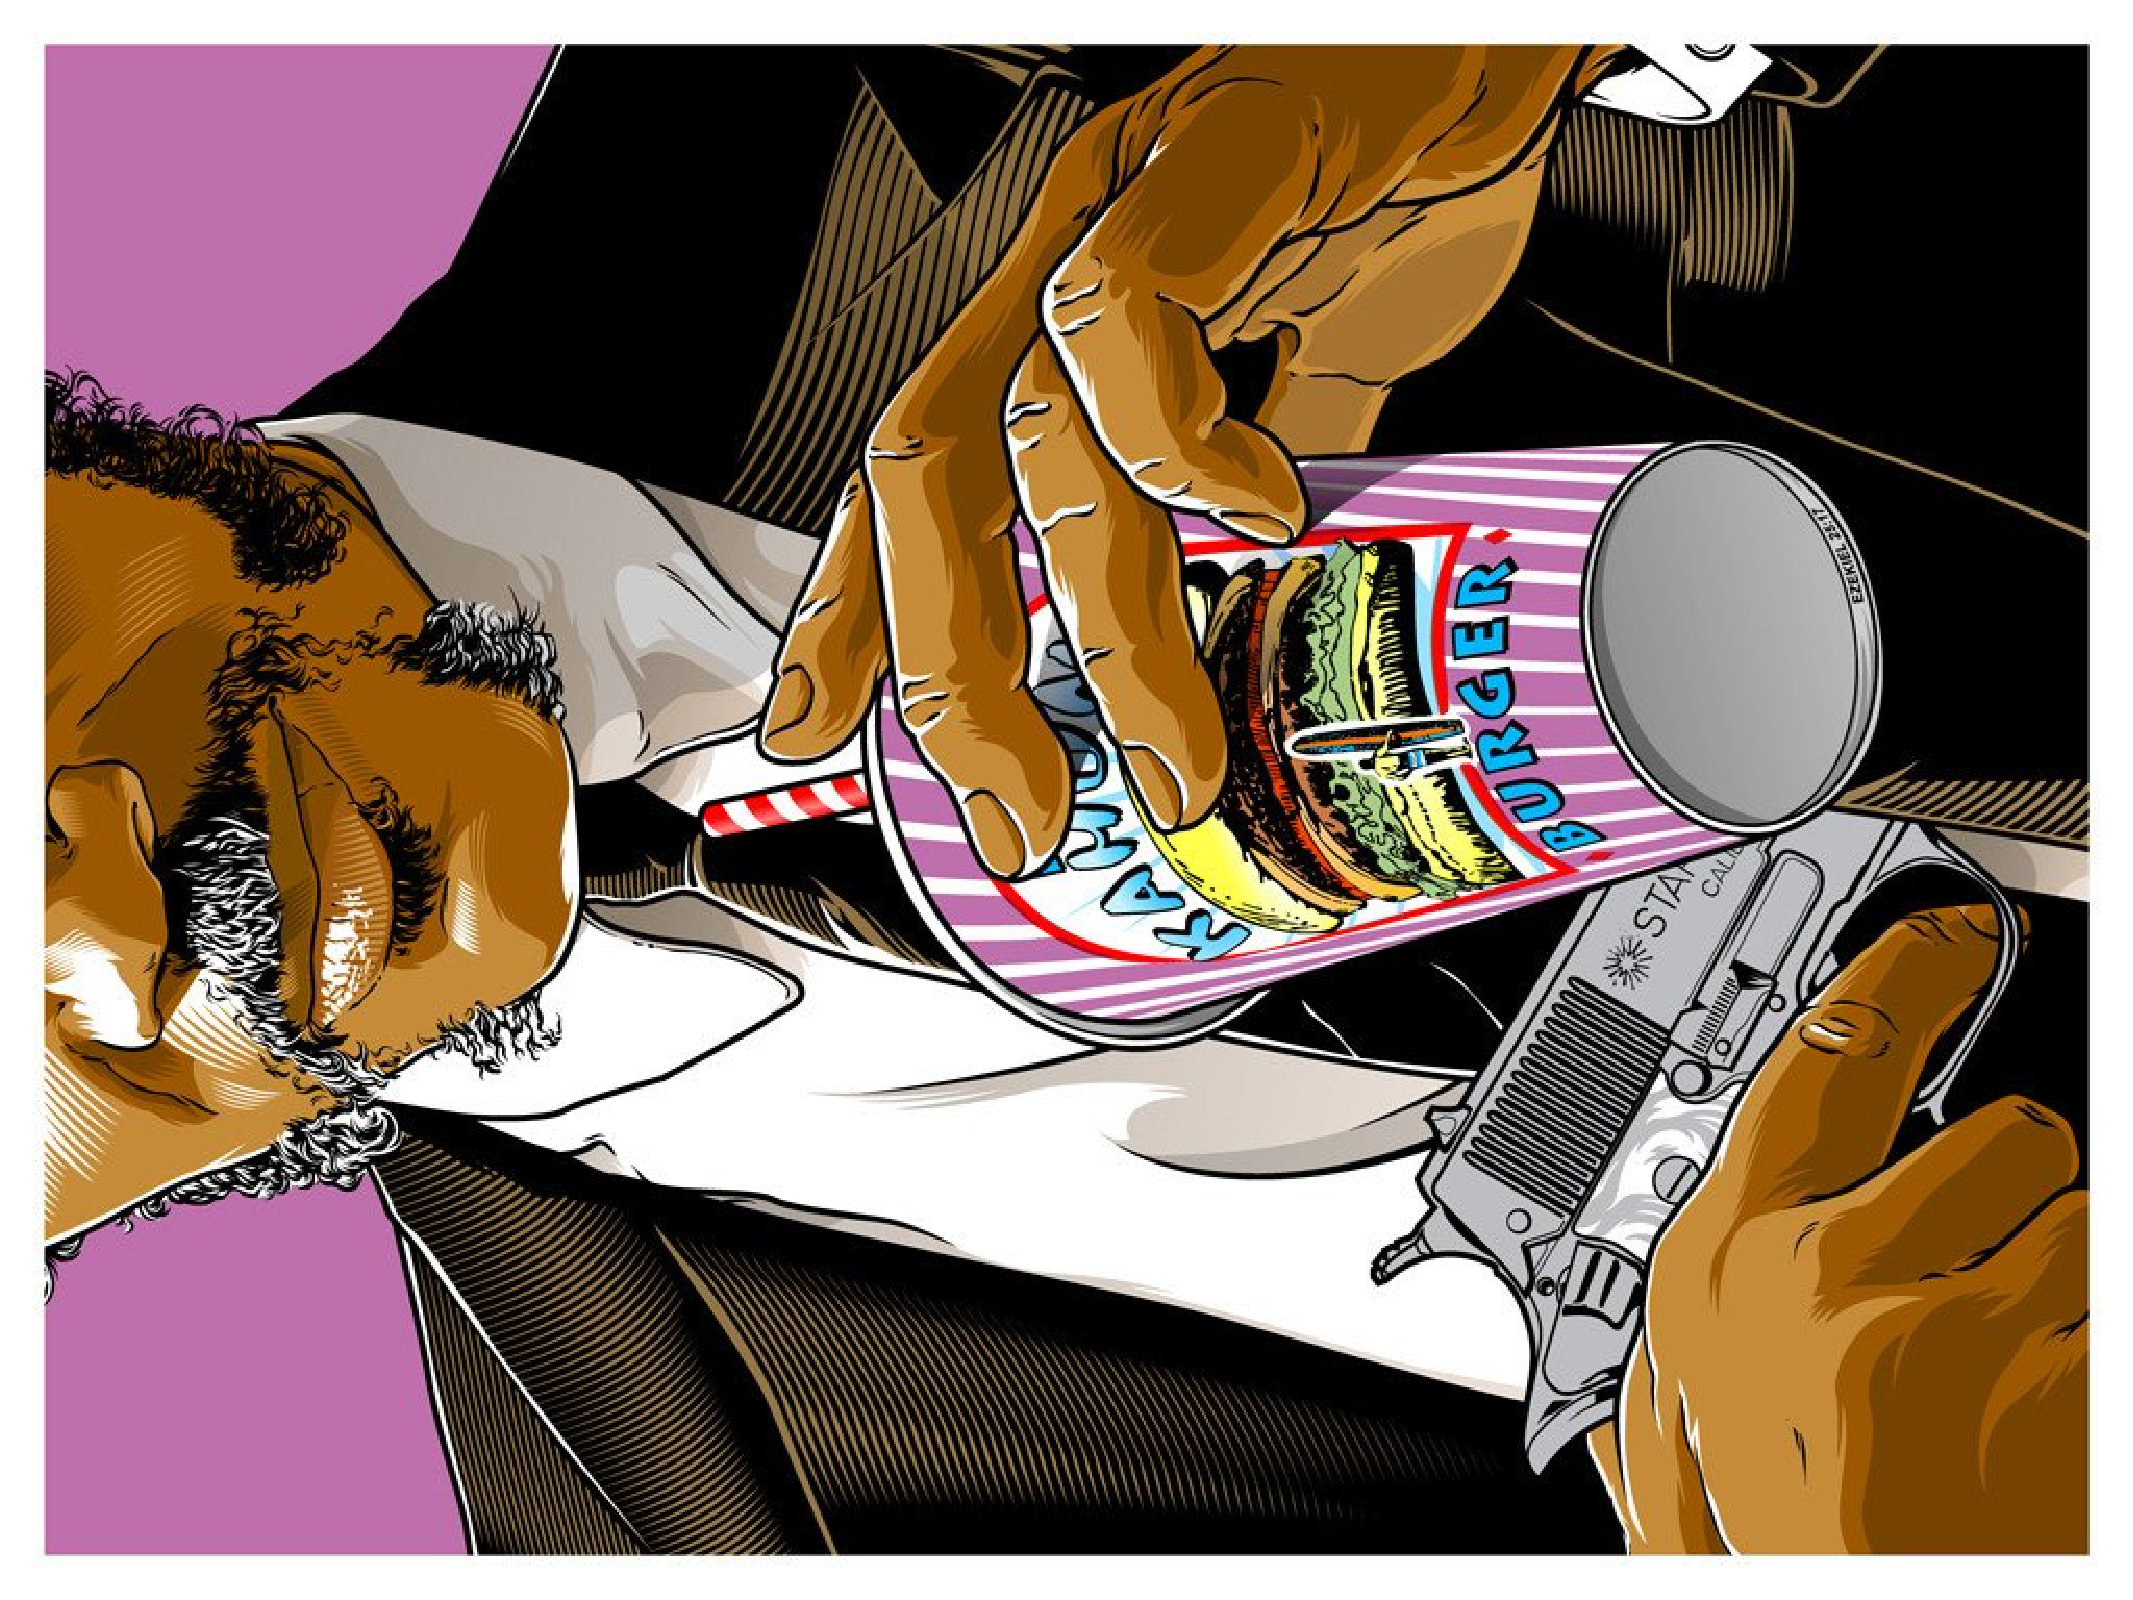
\includegraphics[scale=0.18,angle=270]{pop1.pdf}
\end{minipage}
\hfill
\begin{minipage}[h!]{0.28\linewidth}
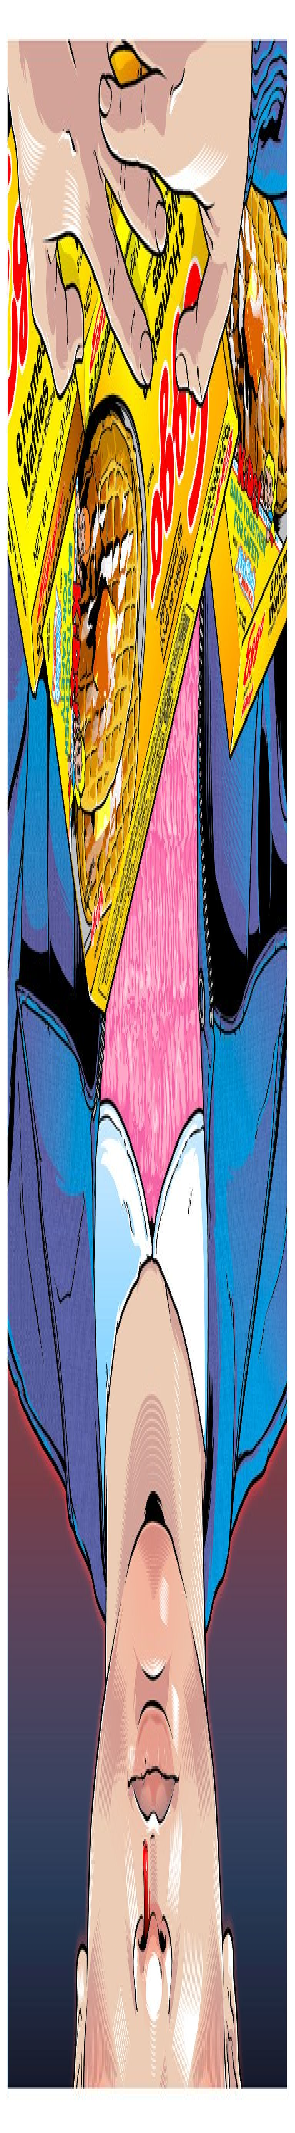
\includegraphics[height=6.5cm,width=4.8cm,angle=180]{pop2.pdf}
\end{minipage}
\hfill
\begin{minipage}[h!]{0.28\linewidth}

\includegraphics[scale=18]{pop3.pdf}
\end{minipage}
\hfill
\begin{minipage}[h!]{0.28\linewidth} 
\includegraphics[scale=0.018]{pop5.pdf}
\end{minipage}
\hfill
\begin{minipage}[h!]{0.28\linewidth} 
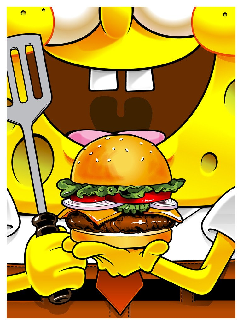
\includegraphics[scale=1.18]{pop8.pdf}
\end{minipage}
\hfill
\begin{minipage}[h!]{0.28\linewidth} 
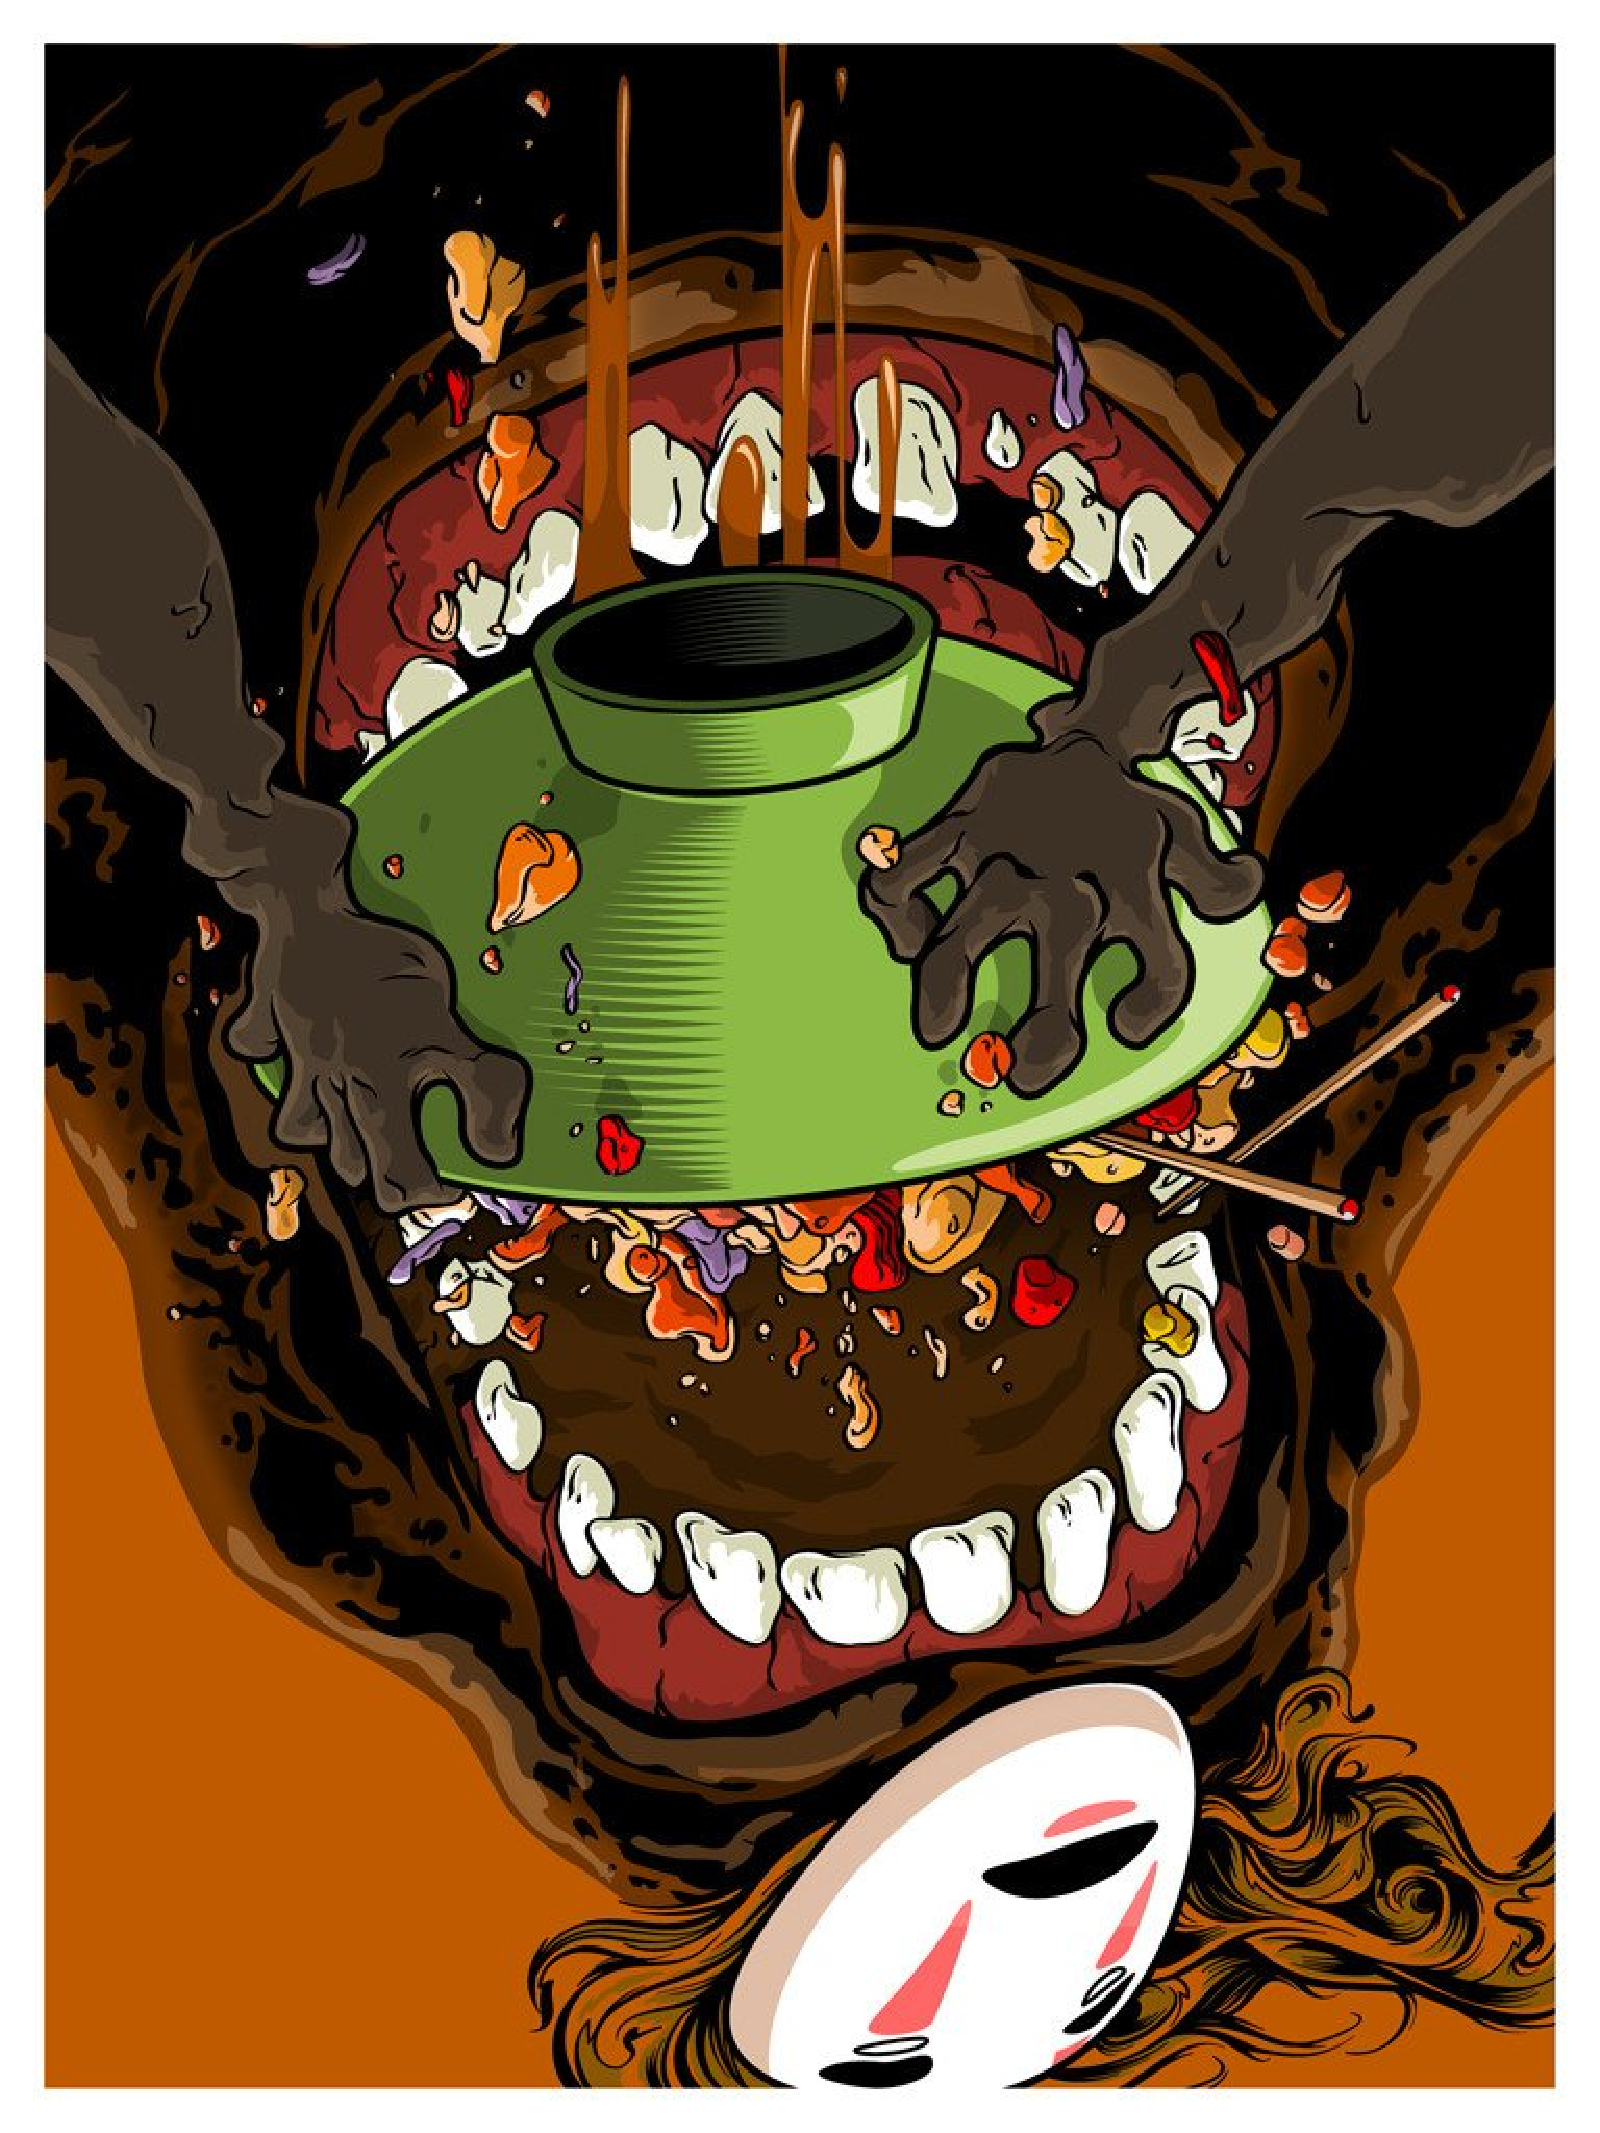
\includegraphics[scale=0.18,angle=180]{pop6.pdf}
\end{minipage}
\caption{Это что, поп арт?}
\end{figure}
\end{document}


